\chapter{Implementation}

\section{Introduction}

This chapter presents the practical implementation of the Infrastructure Command Center, documenting the development process and the final solution. It describes the work environment and tools used during development, presents the three major features that compose the platform, and addresses key technical challenges encountered along the way.

The implementation phase successfully transformed architectural designs into a production-ready platform that centralized FinGenesis's infrastructure management operations.

\section{Work Environment}

The development of the Infrastructure Command Center utilized a set of tools and platforms that facilitated efficient implementation and collaboration throughout the nine sprints.

\subsection{Development Infrastructure}

\textbf{AWS EC2 Instance}: Development was conducted on dedicated AWS EC2 virtual machines provisioned for each team member. This approach ensured consistent development environments and aligned with FinGenesis's cloud-native infrastructure practices.

\textbf{Cursor IDE}: An enhanced version of VS Code with additional features, Cursor served as the primary code editor for both frontend and backend development.

\subsection{Version Control and Deployment}

\textbf{GitLab}: Provided version control for all code repositories and managed the CI/CD pipeline. Every code change was tracked, reviewed, and automatically deployed through GitLab's integrated pipeline system.

\subsection{Project Management and Documentation}

\textbf{Notion}: Served as the central project management platform, tracking sprint backlogs, task progress, and technical documentation. All meeting notes, decisions, and development guidelines were maintained in Notion for easy reference.

\subsection{Communication and Collaboration}

\textbf{Discord}: Facilitated team communication through dedicated channels for different topics. Discord bots provided automated notifications for GitLab pipeline status and scheduled job execution, enabling real-time awareness of deployment activities and system events.

\subsection{API Testing and Debugging}

\textbf{Postman}: Used for testing backend API endpoints, validating request/response formats, and debugging integration issues with GitLab API and Prometheus services.

This work environment provided the necessary tools for efficient development, enabling smooth collaboration and rapid iteration throughout the implementation phase.

\section{Solution Presentation}

This section presents the implemented features of the Infrastructure Command Center, demonstrating how the requirements defined in Chapter 3 were translated into working functionality. The presentation follows the user journey through the platform, starting with the home page and progressing through each major feature.

\subsection{Home Page}

The home page serves as the entry point to the Infrastructure Command Center, providing a clean, intuitive interface that welcomes users and guides them to the platform's main features. The design emphasizes simplicity and ease of navigation, allowing both technical and non-technical users to quickly access the information they need.

The home page includes placeholder sections for features planned for future development as requested by FinGenesis. This forward-looking design ensures the platform can evolve with organizational needs while maintaining a cohesive user experience.

\begin{figure}[H]
    \centering
    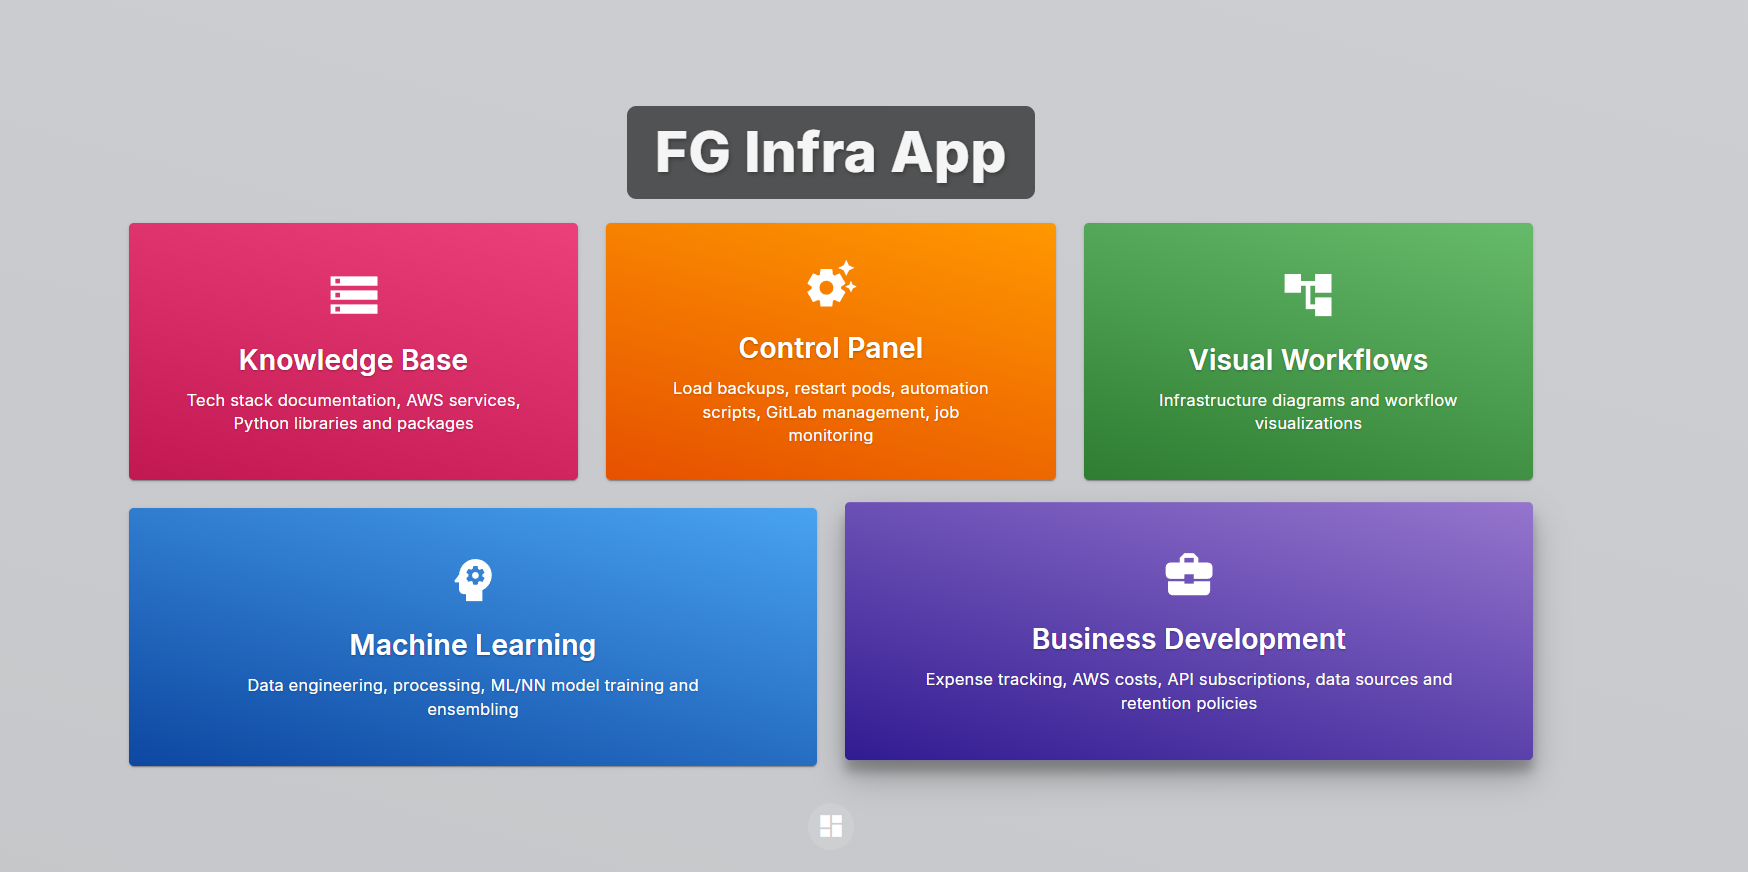
\includegraphics[width=\textwidth]{images/home.png}
    \caption{Infrastructure Command Center Home Page}
    \label{fig:home_page}
\end{figure}

\subsection{Dynamic Visual Workflows}

The Visual Workflows feature provides an interactive representation of FinGenesis's main application architecture. Its purpose is to help engineers, stakeholders, and external parties quickly understand the system's structure and monitor service health in real-time without requiring deep technical knowledge.

\textbf{Implementation Overview:}

The visualization was built using ReactFlow, a specialized library for creating node-based diagrams. Custom node components were designed for each service type, with interactive click handlers enabling navigation between different views. Service health status is fetched from monitoring systems and displayed through color-coded indicators (green for up, red for down, yellow for error states).

\textbf{Three-Level Visualization:}

The feature provides three interconnected views that progressively reveal architectural details:

\textbf{Overview Diagram}: The default view presents the architecture organized into four main sections: Client Application, Market Data, ML Engine, and Backend Services. This high-level view provides immediate understanding of the system's major components and their relationships.

\begin{figure}[H]
    \centering
    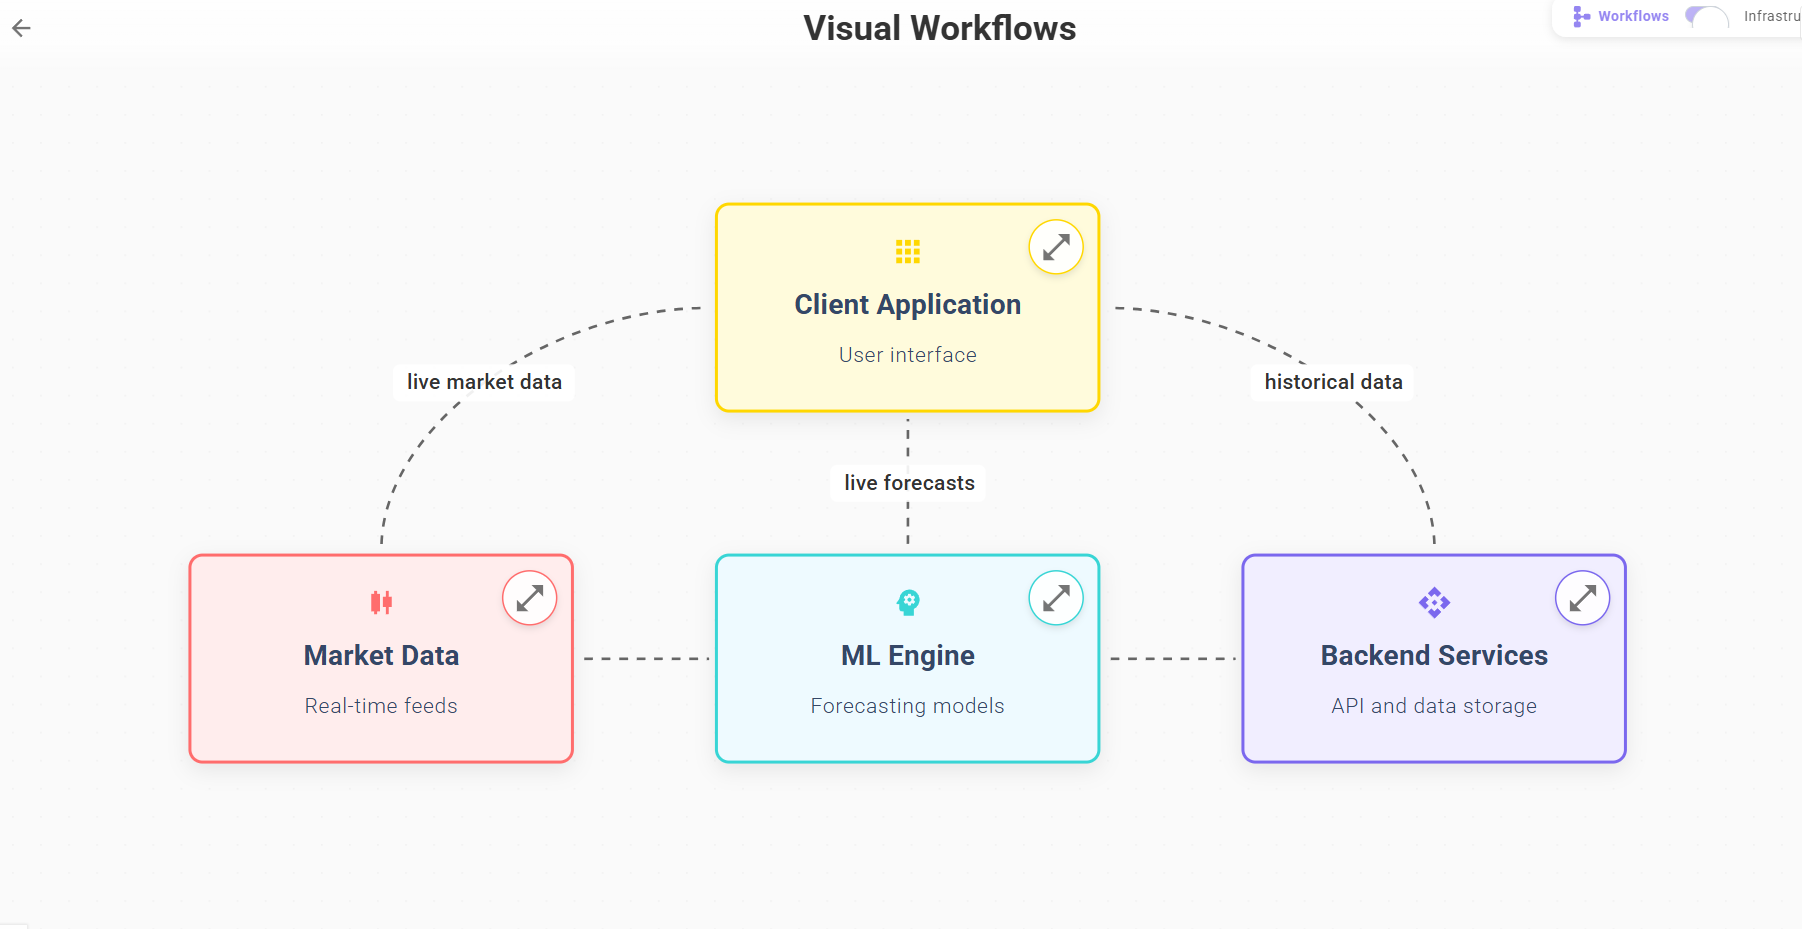
\includegraphics[width=\textwidth]{images/workflow_overview.png}
    \caption{Visual Workflows - Overview Diagram}
    \label{fig:workflow_overview}
\end{figure}

\textbf{Detailed Section View}: Clicking on any of the four main sections navigates to a detailed view showing all services within that section, their internal workflows, and real-time health indicators. This allows users to focus on specific subsystems and quickly identify problematic services.

\begin{figure}[H]
    \centering
    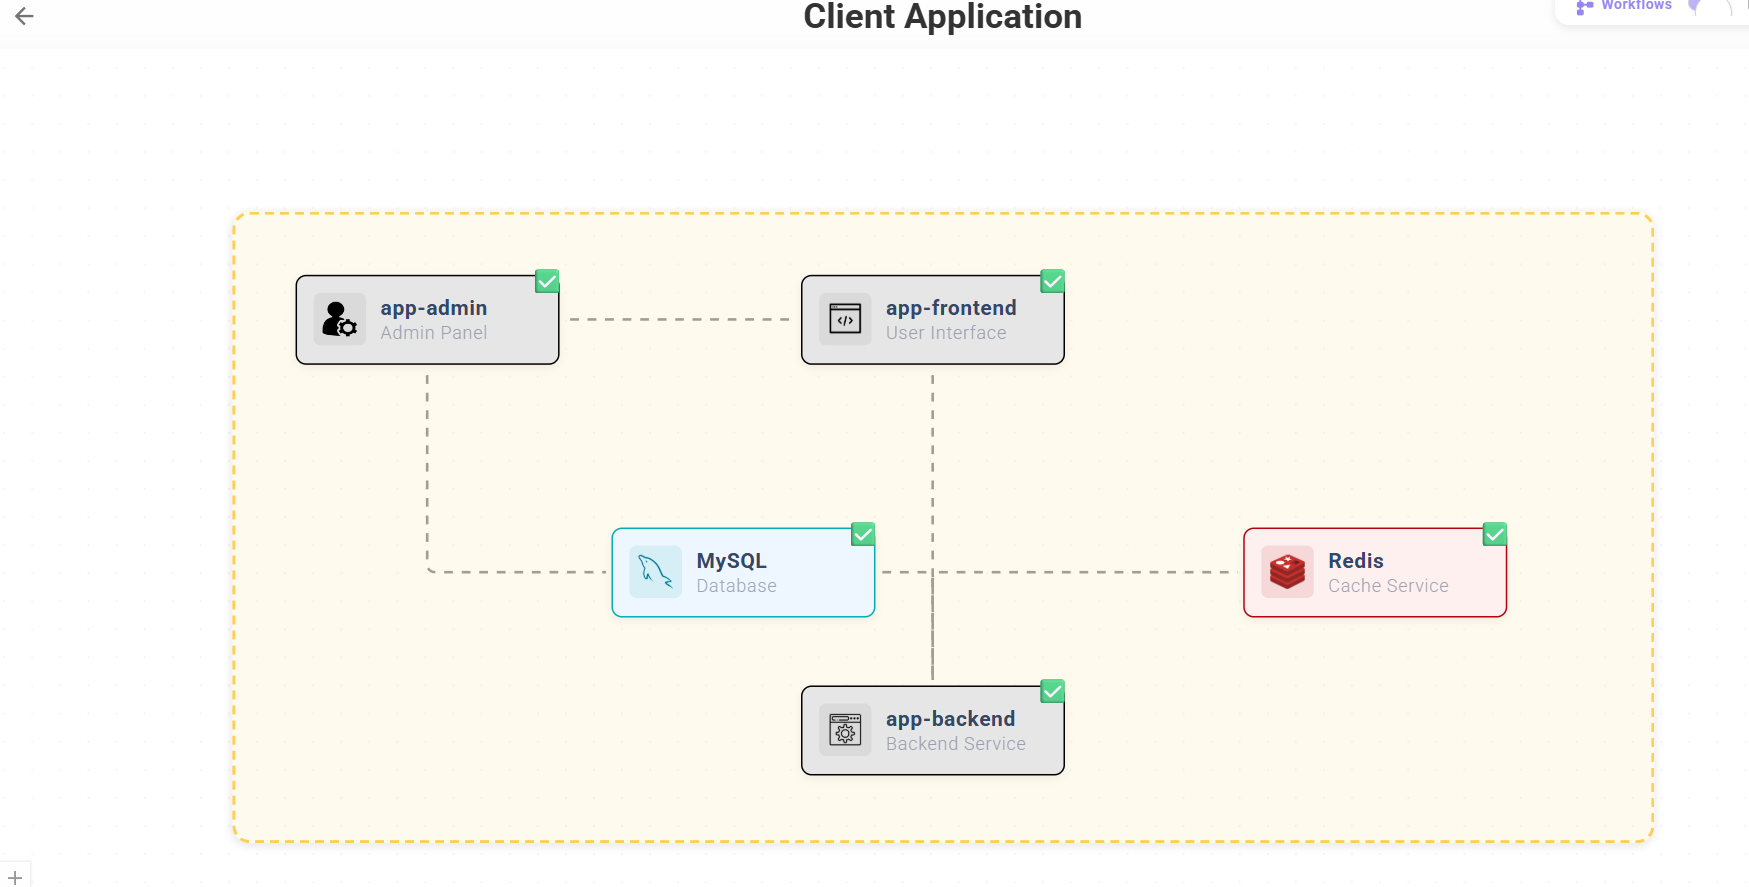
\includegraphics[width=\textwidth]{images/workflow_detail2.png}
    \caption{Visual Workflows - Detailed Section View}
    \label{fig:workflow_detail2}
\end{figure}

\textbf{Complete Detailed Diagram}: A toggle switch enables users to view all four sections with all their services in a single comprehensive diagram. This view is particularly useful for understanding cross-section dependencies and overall system health at a glance.

\begin{figure}[H]
    \centering
    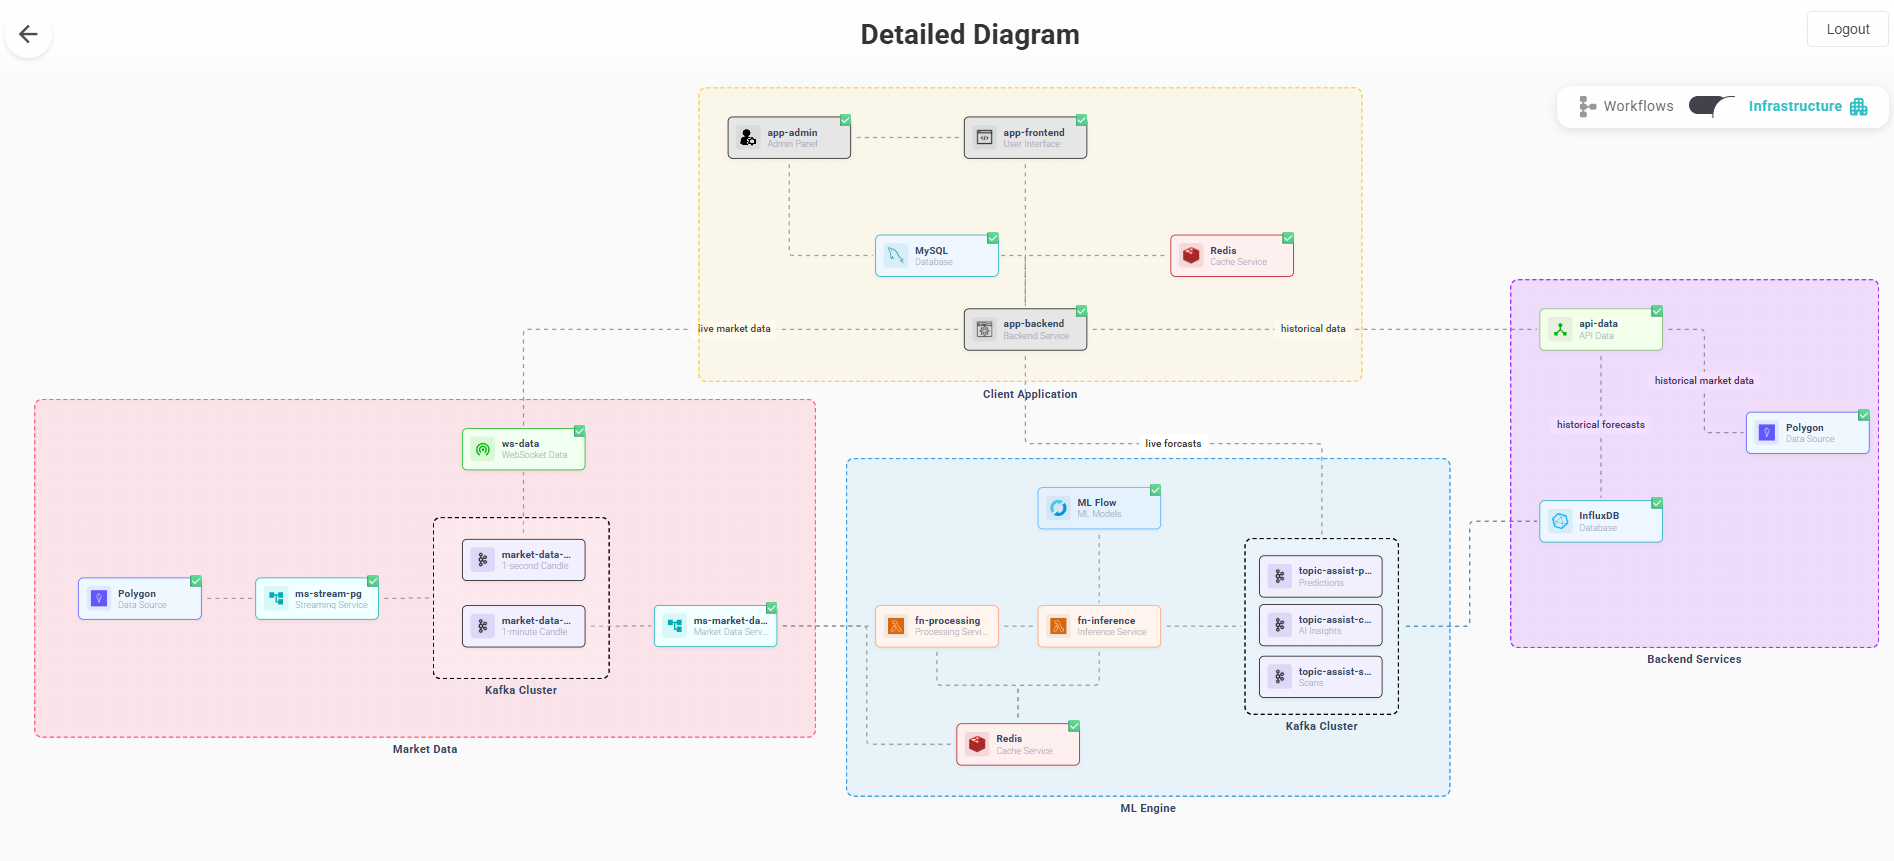
\includegraphics[width=\textwidth]{images/workflow_complete.png}
    \caption{Visual Workflows - Complete Detailed Diagram}
    \label{fig:workflow_complete}
\end{figure}

\textbf{Health Status Indicators}: Each service node displays a real-time status indicator with three possible states: up (operational), down (unavailable), or error (experiencing issues). These visual cues enable immediate identification of system problems without requiring manual log inspection or metric analysis.

The combination of interactive navigation, progressive detail revelation, and real-time health monitoring makes infrastructure architecture accessible to both technical teams and non-technical stakeholders.

\begin{figure}[H]
    \centering
    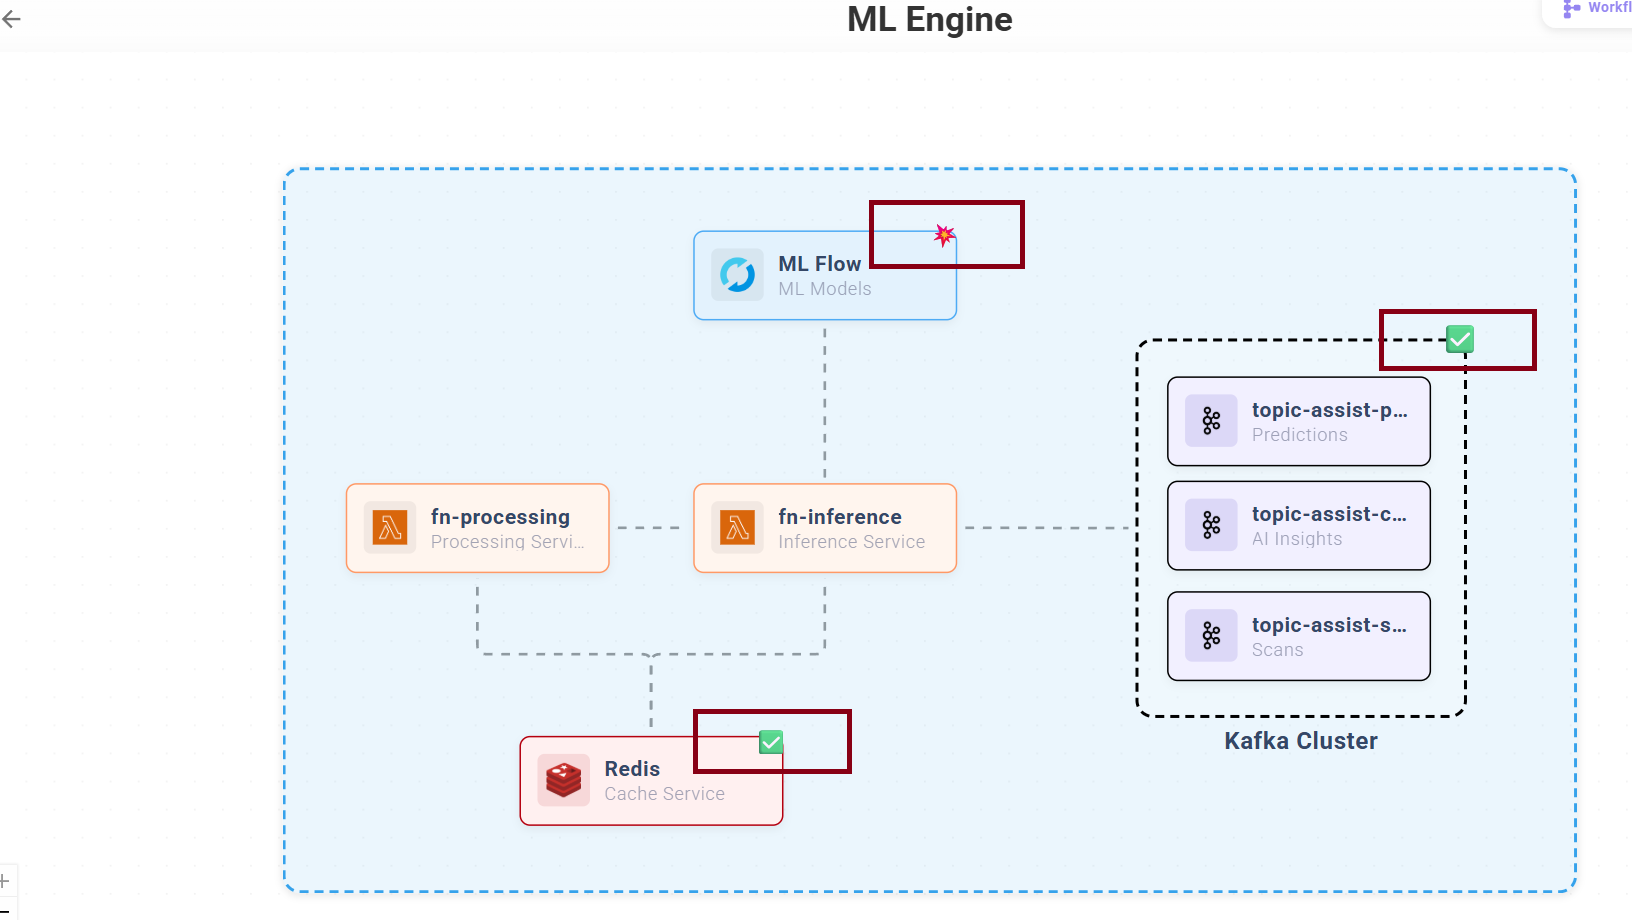
\includegraphics[width=\textwidth]{images/workflow_detail3.png}
    \caption{Visual Workflows - Health Status Indicators}
    \label{fig:workflow_detail3}
\end{figure}

\subsection{Control Panel}

The Control Panel is the most efficient and important feature of the Infrastructure Command Center. Its purpose is to eliminate the need for navigating GitLab's interface directly, automate common repository management tasks, and provide developers with visibility into all company repositories without requiring individual access permissions. This centralized view enables developers to understand the state of infrastructure repositories and perform on-the-fly actions efficiently.

\textbf{Implementation Overview:}

The Control Panel is built using GitLab API v4 to fetch repository information, pipeline statuses, and merge request data. The backend implements caching strategies to improve loading performance when handling 40+ repositories, significantly reducing response times from initial load to subsequent requests. The frontend displays this information in an organized, searchable list with intelligent action buttons determined by backend logic that evaluates branch state, pipeline status, and merge request availability.

\textbf{Repository List Display:}

The main interface presents all company repositories in a comprehensive list. Each repository entry displays:

\begin{itemize}
    \item Repository name and group
    \item Number of extra branches (branches other than main)
    \item Count of open merge requests
    \item Latest pipeline information (status, stage, and branch)
    \item Available actions based on current repository state
\end{itemize}

\begin{figure}[H]
    \centering
    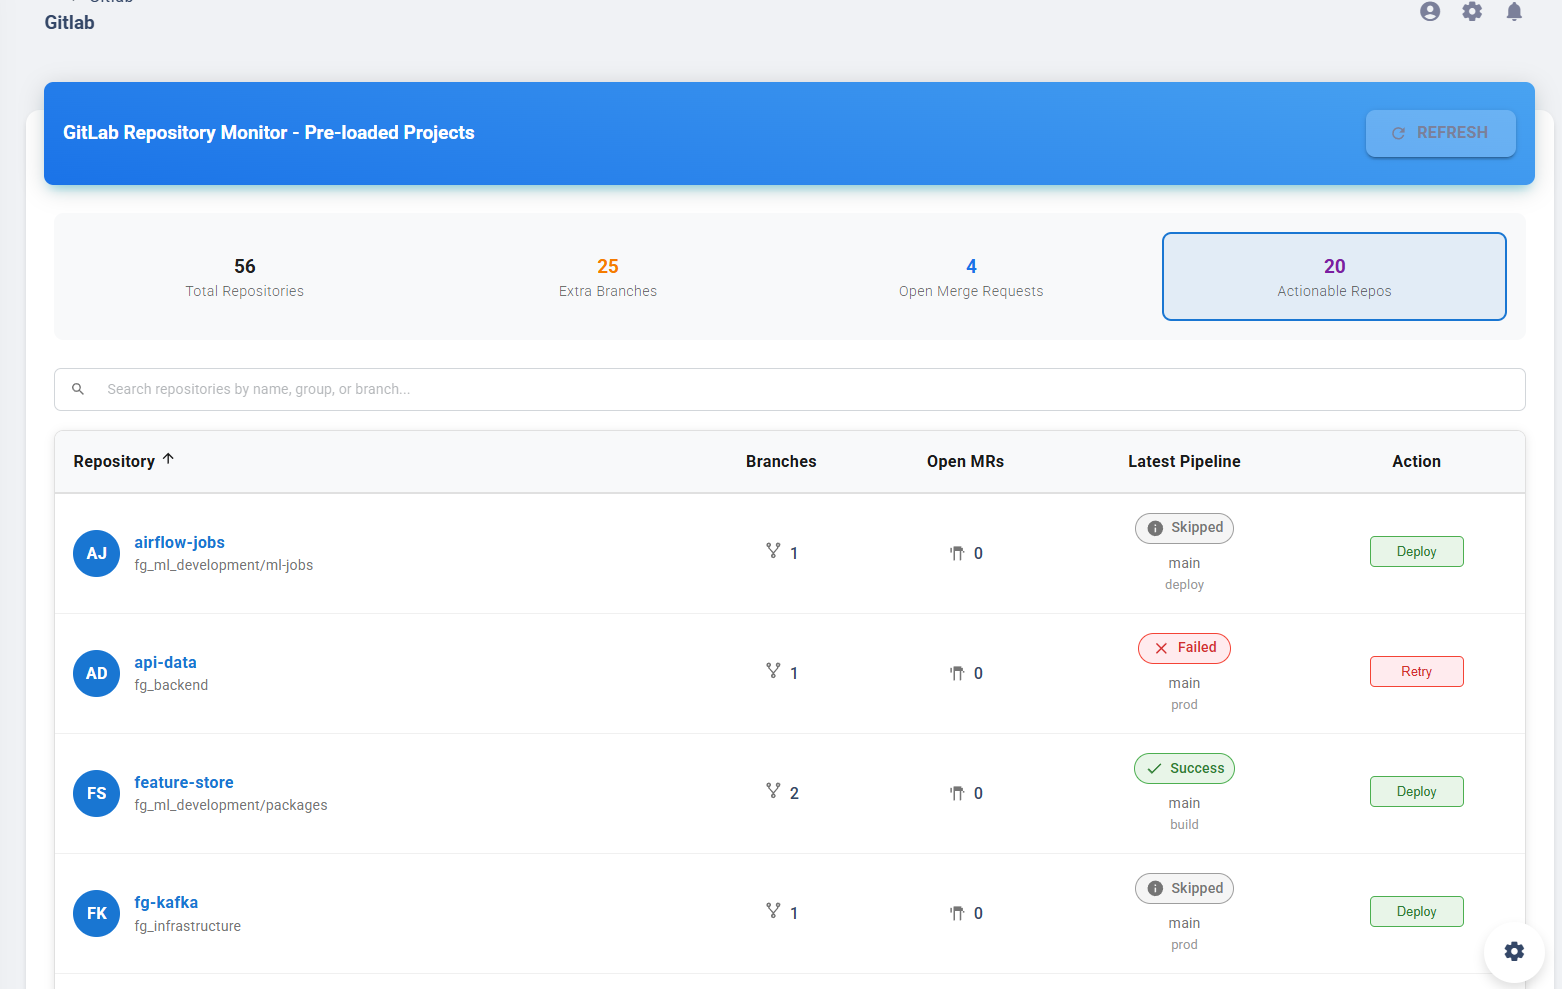
\includegraphics[width=\textwidth]{images/repos_list.png}
    \caption{Control Panel - Repository List}
    \label{fig:control_panel_list}
\end{figure}

\textbf{Sorting and Filtering:}

The Control Panel provides flexible data organization to help users quickly locate repositories of interest:

\textbf{Sorting Options:}
\begin{itemize}
    \item By name (alphabetically)
    \item By number of branches (numerical order)
    \item By pipeline status (grouped by passed/failed/running)
\end{itemize}

\textbf{Filtering Options:}
\begin{itemize}
    \item Open MRs: Shows only repositories with open merge requests
    \item Actionable Repos: Shows only repositories with available actions
\end{itemize}

\textbf{Dynamic Search:} A search bar filters repositories in real-time as users type, enabling quick location of specific projects.

\textbf{Repository Actions:}

Clicking on a repository name opens its GitLab page directly. Beyond navigation, the Control Panel provides actionable buttons that appear based on intelligent logic:

\textbf{Action Display Logic:}
\begin{itemize}
    \item If branch is not main and pipeline failed → Display \textbf{Retry} button
    \item If branch is not main and pipeline passed → Display \textbf{Open MR} button
    \item If branch is not main, pipeline passed, and MR already exists → Display \textbf{MR Already Open} indicator
    \item If branch is main and pipeline failed → Display \textbf{Retry} button
    \item If branch is main, pipeline passed, and manual deployment job available → Display \textbf{Deploy} button
    \item If branch is main, pipeline passed, and project already deployed → Display \textbf{Already Deployed} indicator
\end{itemize}

\textbf{Merge Request Management:}

The Control Panel streamlines merge request workflows through modal interfaces:

\textbf{Opening Merge Requests:} Clicking the "Open MR" button displays a modal where users can enter the merge request title, description, and choose whether to delete the source branch after merging.

\begin{figure}[H]
    \centering
    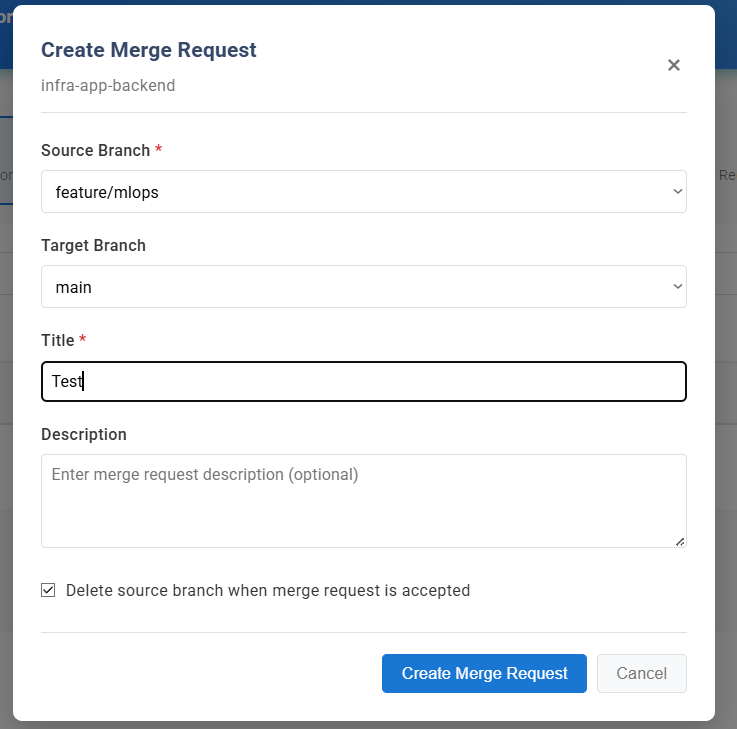
\includegraphics[width=0.8\textwidth]{images/createMR.png}
    \caption{Control Panel - Open Merge Request Modal}
    \label{fig:open_mr_modal}
\end{figure}

\textbf{Accepting or Rejecting Merge Requests:} When reviewing merge requests, users can accept them directly or reject them with an explanatory comment. This functionality enables code review workflows without leaving the Infrastructure Command Center.

\begin{figure}[H]
    \centering
    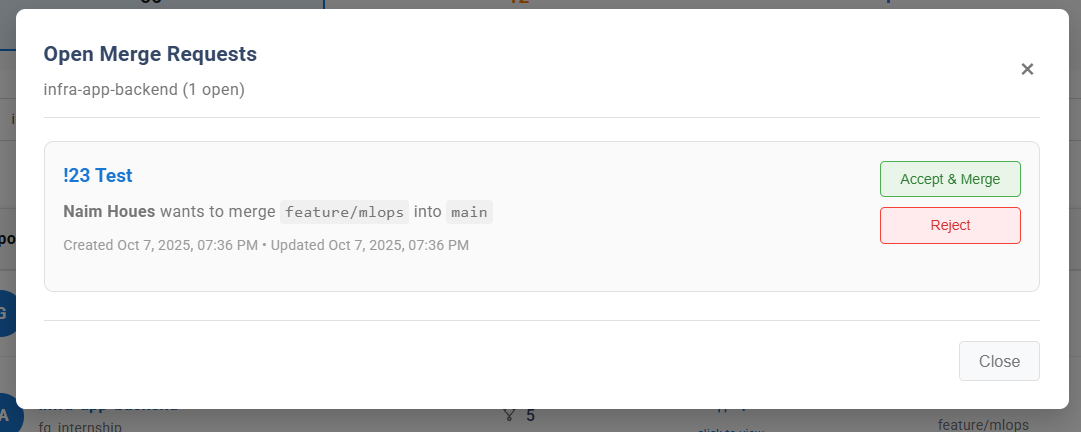
\includegraphics[width=0.8\textwidth]{images/acceptMR.png}
    \caption{Control Panel - Accept/Reject Merge Request Modal}
    \label{fig:accept_mr_modal}
\end{figure}

\textbf{Pipeline Operations:}

Users can trigger pipeline deployments and retry failed pipelines directly from the repository list. These actions execute immediately, with status updates reflected in real-time as the backend polls GitLab for updated pipeline states.

The Control Panel transforms repository management from a multi-step, permission-dependent process into a streamlined, accessible operation. By consolidating visibility and actions into a single interface, it significantly reduces the time engineers spend on routine deployment and merge request tasks.

\subsection{ML Metrics Monitoring}

The ML Metrics Monitoring section provides comprehensive performance tracking for FinGenesis's deployed machine learning models. Its purpose is to help data scientists and engineers monitor model accuracy, detect performance drift, and ensure prediction quality meets business requirements. This feature is custom-built to display the specific metrics and visualizations that FinGenesis needs, presented in the format most useful for their operations.

\textbf{Implementation Overview:}

The monitoring system is built using Recharts for visualization and processes model performance data loaded from CSV files. The backend calculates rolling accuracy metrics across different time windows, aggregates data for multi-model views, and provides real-time performance summaries. The frontend presents this information through interactive charts and status cards that update based on user-selected configurations.

\textbf{Dashboard Overview:}

The monitoring dashboard provides immediate visibility into model performance through summary cards and configurable views:

\begin{figure}[H]
    \centering
    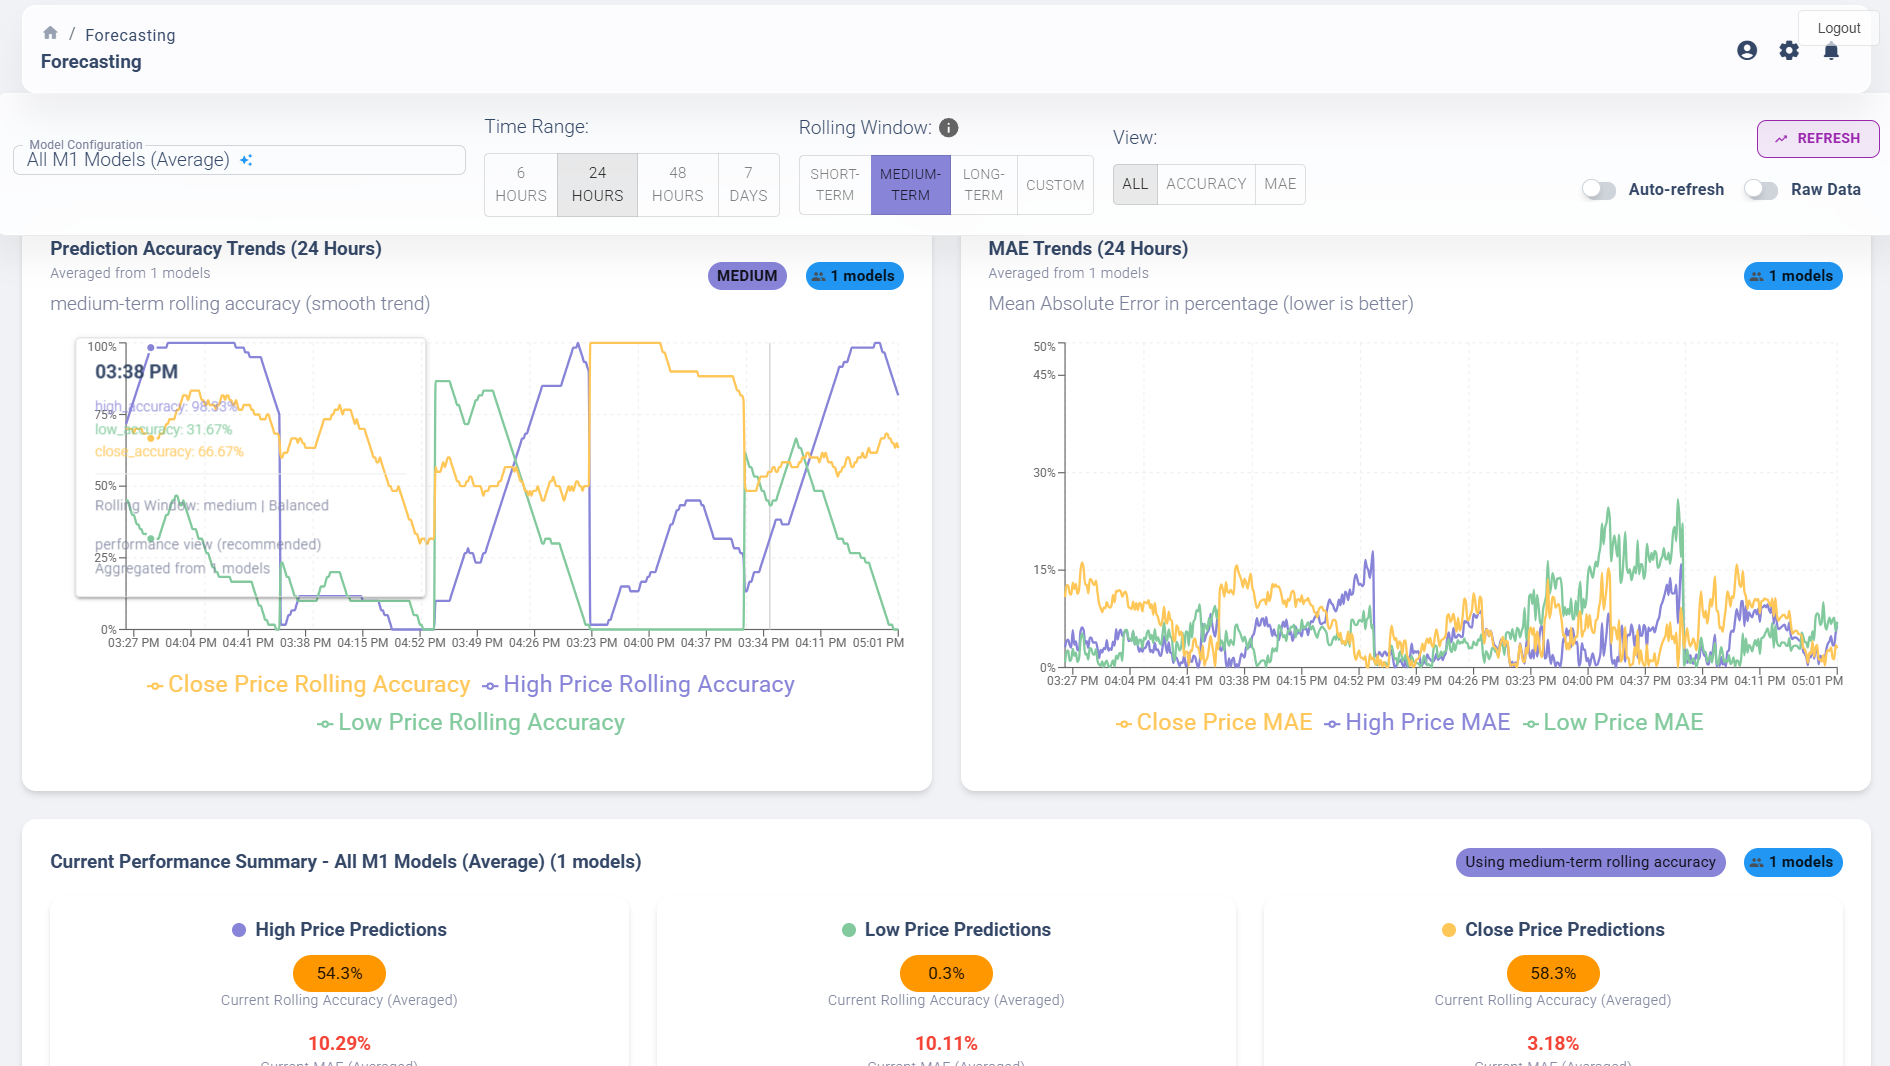
\includegraphics[width=\textwidth]{images/mlops.png}
    \caption{ML Metrics Monitoring Dashboard}
    \label{fig:mlops_dashboard}
\end{figure}

\textbf{Summary Metrics:}

Four key indicators provide at-a-glance performance status:

\begin{itemize}
    \item \textbf{Total Configurations}: Number of available model configurations (individual models and aggregated views)
    \item \textbf{Average Accuracy (24h)}: Overall prediction accuracy across all selected models
    \item \textbf{Average MAE (24h)}: Mean Absolute Error averaged across predictions (lower values indicate better performance)
    \item \textbf{Healthy Models}: Count of models meeting performance thresholds based on accuracy criteria
\end{itemize}

\textbf{Configuration and Time Controls:}

Users can customize their view through several control options:

\textbf{Model Configuration Selector}: A dropdown menu allows selection between individual models or aggregated multi-model views, enabling comparison across different prediction configurations.

\textbf{Time Range Selection}: Four preset time ranges (6 hours, 24 hours, 48 hours, 7 days) let users zoom into recent performance or analyze longer-term trends.

\textbf{Rolling Window Selection}: Three window options (short-term, medium-term, long-term) control the smoothing level of accuracy calculations. Rolling accuracy averages predictions over a time window, providing smooth trends rather than volatile binary accuracy (0\% or 100\%) that would result from individual predictions.

\textbf{View Filter}: Options to display all metrics, accuracy only, or MAE only, reducing visual clutter when focusing on specific performance aspects.

\textbf{Prediction Accuracy Trends:}

The accuracy chart visualizes how well models predict High, Low, and Close prices over time. Accuracy represents the percentage of predictions that correctly forecast price movements. The rolling accuracy calculation smooths out short-term volatility, revealing underlying performance trends that help identify gradual drift or sudden degradation.

\begin{figure}[H]
    \centering
    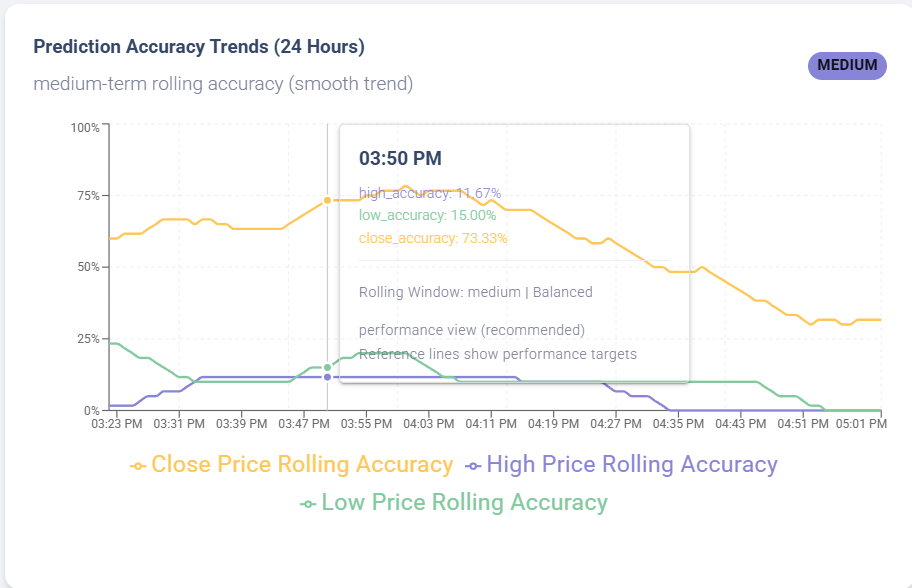
\includegraphics[width=\textwidth]{images/accuracy.png}
    \caption{Prediction Accuracy Trends with Rolling Window}
    \label{fig:accuracy_trends}
\end{figure}

Three colored lines represent different prediction types:
\begin{itemize}
    \item High Price (purple): Accuracy of predicting maximum price points
    \item Low Price (green): Accuracy of predicting minimum price points  
    \item Close Price (orange): Accuracy of predicting closing prices
\end{itemize}

\textbf{MAE Trends:}

The MAE (Mean Absolute Error) chart displays prediction error magnitude over time. MAE measures the average absolute difference between predicted and actual values, expressed as a percentage. Lower MAE values indicate more accurate predictions. This metric is particularly important because a model can have high accuracy (correct direction) but poor precision (large error magnitude).

\begin{figure}[H]
    \centering
    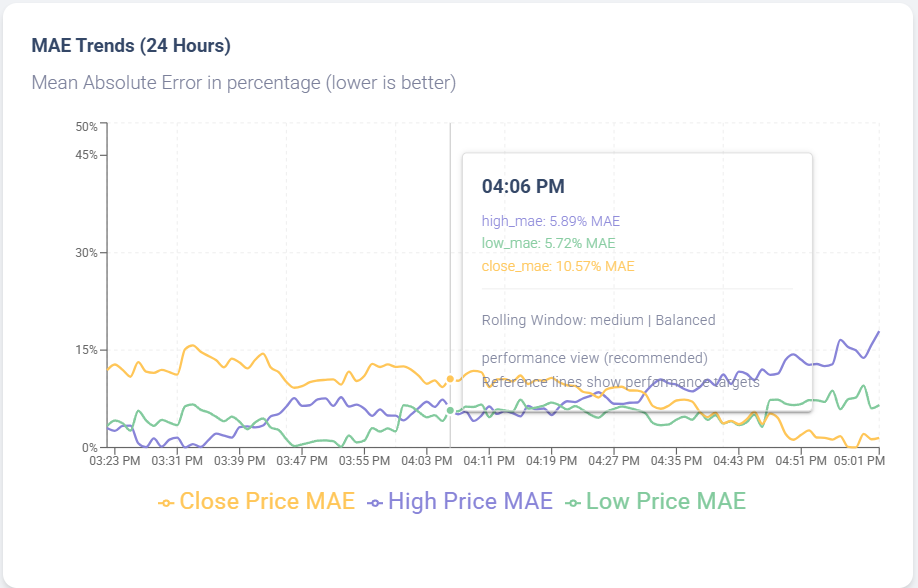
\includegraphics[width=\textwidth]{images/mae.png}
    \caption{MAE Trends - Lower is Better}
    \label{fig:mae_trends}
\end{figure}

\textbf{Performance Summary Cards:}

Three detailed cards provide comprehensive metrics for each prediction type (High, Low, Close):

\begin{figure}[H]
    \centering
    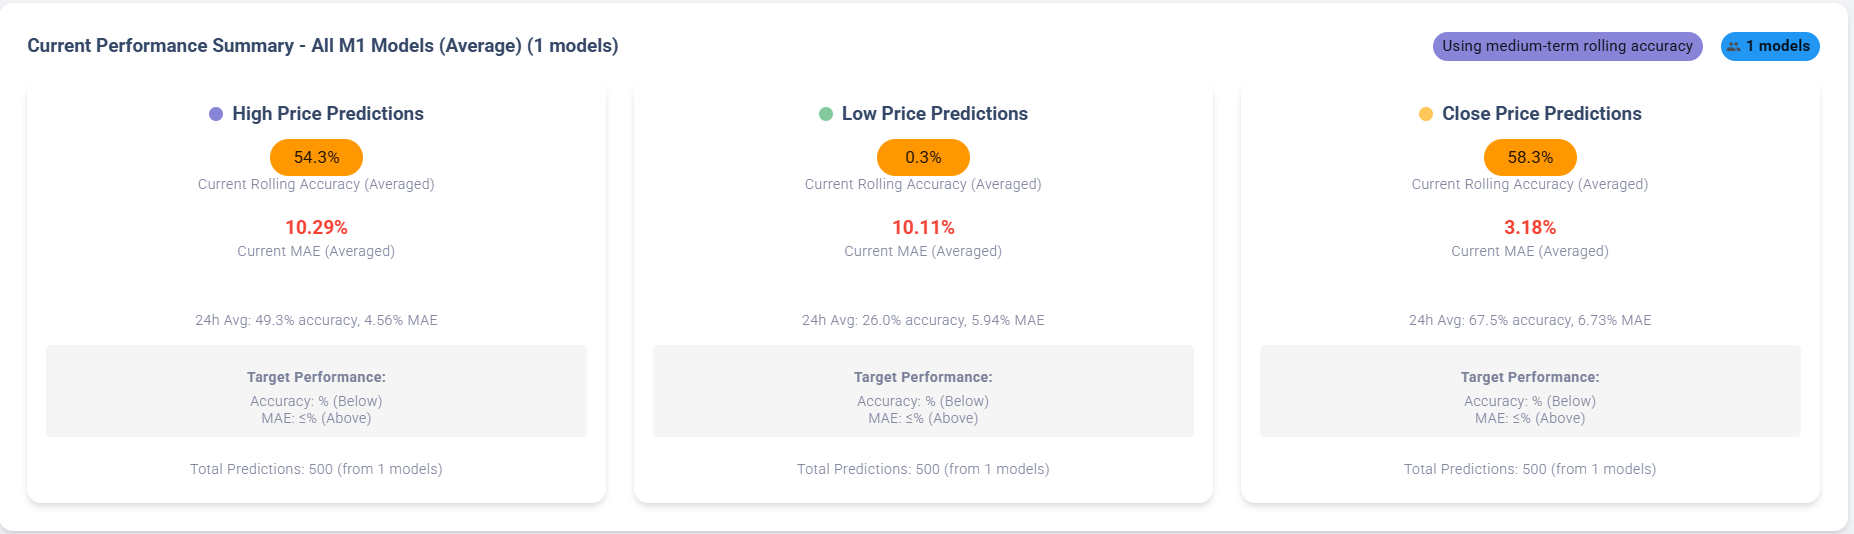
\includegraphics[width=\textwidth]{images/cards.png}
    \caption{Current Performance Summary Cards}
    \label{fig:performance_cards}
\end{figure}

Each card displays:
\begin{itemize}
    \item \textbf{Current Rolling Accuracy}: Latest smoothed accuracy value
    \item \textbf{Current MAE}: Most recent error measurement
    \item \textbf{24h Averages}: Performance over the past day for context
    \item \textbf{Target Performance}: Reference benchmarks showing whether current performance meets, exceeds, or falls below established targets
    \item \textbf{Total Predictions}: Number of predictions included in the analysis
\end{itemize}

\textbf{Reference Target Comparison:}

The Target Performance section compares actual metrics against established benchmarks. Visual indicators show whether current accuracy meets target thresholds and whether MAE stays within acceptable ranges. This feature enables quick identification of models requiring attention or retraining.

\textbf{Real-time Monitoring:}

The dashboard automatically refreshes data at regular intervals, ensuring engineers always see current model performance. The combination of rolling accuracy smoothing, configurable time windows, and reference target comparisons provides both immediate alerts for critical issues and long-term trend analysis for proactive maintenance.

The ML Metrics Monitoring section transforms raw prediction data into actionable insights, enabling FinGenesis's team to maintain high-quality model performance and respond quickly to degradation or drift.

\section{Challenges}

The development of the Infrastructure Command Center presented several challenges that required careful problem-solving and technical decision-making. This section discusses the learning challenges encountered as a junior developer and two major technical obstacles that significantly impacted the project's success.

\subsection{General Learning Challenges}

As a junior developer working on a production-scale project, the Infrastructure Command Center presented a steep learning curve across multiple dimensions. The project required mastering several new technologies simultaneously: React for frontend development, FastAPI for backend services, Docker and Kubernetes for deployment, and GitLab CI/CD for automation. Each technology brought its own concepts, best practices, and debugging challenges.

Working in FinGenesis's professional environment added another layer of complexity. The codebase followed enterprise-level standards, requiring adherence to established conventions, code review processes, and deployment protocols. Understanding the existing infrastructure architecture, integrating with production systems, and maintaining compatibility with company standards demanded continuous learning and adaptation.

The fast-paced sprint cycles meant there was limited time to master each technology before moving to implementation. Debugging issues often required understanding how multiple systems interacted frontend state management, backend API orchestration, external service integrations, and containerized deployments. This required developing systematic problem-solving approaches and learning to leverage documentation, community resources, and mentor guidance effectively.

Despite these challenges, the structured Agile methodology and regular code reviews provided valuable learning opportunities. Each sprint retrospective identified areas for improvement, and daily standups helped maintain alignment with project goals. The experience of building a complete, production-deployed platform while learning advanced technologies simultaneously proved to be an intensive but highly effective learning process.

\subsection{Challenge \#1: Visualizing Complex Infrastructure Workflows}

\textbf{The Problem:}

Creating an effective visualization for FinGenesis's complex, multi-service architecture presented a significant challenge. The visualization needed to be interactive and explorable, maintainable as the system evolved, and clear for both technical and non-technical stakeholders. Traditional approaches like static diagrams (PNG/SVG) became outdated quickly and required manual updates through tools like Draw.io or Lucidchart. The system's complexity with 10+ microservices across multiple deployment environments demanded a solution that could represent data flow, service dependencies, and real-time health status dynamically.

\textbf{Solution Evaluation:}

Several visualization libraries were evaluated based on their suitability for the project's requirements:

\begin{table}[H]
\centering
\caption{Visualization Library Comparison}
\resizebox{\textwidth}{!}{
\begin{tabular}{|l|l|l|l|}
\hline
\textbf{Solution} & \textbf{Pros} & \textbf{Cons} & \textbf{Verdict} \\ \hline
Static Images & Simple, no dependencies & Not interactive, hard to maintain & Rejected \\ \hline
D3.js & Powerful, flexible & Steep learning curve, verbose code & Too complex \\ \hline
Mermaid.js & Code-based, simple syntax & Limited interactivity, styling constraints & Limited \\ \hline
Cytoscape.js & Great for graphs & Complex API, overkill for workflows & Overcomplicated \\ \hline
React Flow & React-native, interactive, extensible & Learning curve for flow concepts & Selected \\ \hline
\end{tabular}
}
\end{table}

\textbf{Why React Flow Won:}

React Flow emerged as the optimal choice for several key reasons:

\begin{itemize}
    \item \textbf{Native React Integration}: Seamlessly integrated with the existing React codebase using familiar component patterns and state management
    \item \textbf{Built-in Interactivity}: Provided drag-and-drop nodes, zoom and pan controls, node selection, and edge routing without requiring custom implementation
    \item \textbf{Customization Power}: Enabled custom node types for different service categories (API gateways, databases, microservices) with tailored styling and behavior
    \item \textbf{Performance Optimization}: Built-in virtualization handled large graphs smoothly, efficiently managing 100+ nodes with responsive rendering
    \item \textbf{Developer Experience}: Excellent documentation, active community support, and regular updates reduced implementation time and debugging complexity
\end{itemize}

\textbf{Implementation Results:}

The React Flow implementation transformed infrastructure visualization from a static, maintenance-heavy process into a dynamic, interactive experience:

\textbf{Before (Static Diagrams):}
\begin{itemize}
    \item Manual updates required for every infrastructure change
    \item No interactivity or ability to explore service relationships
    \item Difficult to show different views or detail levels
    \item Time-consuming maintenance and version synchronization
\end{itemize}

\textbf{After (React Flow):}
\begin{itemize}
    \item \checkmark\ Interactive exploration with zoom, pan, and click navigation
    \item \checkmark\ Dynamic updates from real monitoring data
    \item \checkmark\ Custom node types representing different service categories
    \item \checkmark\ Easy addition or removal of services without redesigning layouts
    \item \checkmark\ Professional, modern interface with responsive performance
\end{itemize}


\textbf{Measurable Improvements:}

\begin{itemize}
    \item \textbf{Development Time}: 2 days (compared to estimated 5+ days with D3.js)
    \item \textbf{Code Efficiency}: Approximately 300 lines of code (versus 1000+ for custom solutions)
    \item \textbf{Maintenance Overhead}: Minutes to update (versus hours with static diagram tools)
\end{itemize}

The React Flow solution successfully balanced technical capability with implementation efficiency, delivering a visualization system that met all project requirements while remaining maintainable and scalable for future infrastructure growth.

\clearpage

\subsection{Challenge \#2: GitLab Repository Performance Issues}

\textbf{The Problem:}

One of the most critical challenges encountered was severe performance degradation when fetching data for FinGenesis's 40+ GitLab repositories. The initial implementation used sequential API calls, resulting in unacceptable load times exceeding 30 seconds. This created a poor user experience with frozen interfaces, risked hitting GitLab's API rate limits, and resulted in redundant data fetching on every request.

The performance bottleneck stemmed from the architecture's approach: for each repository, the system made separate API calls to fetch pipeline status, branch information, and merge request data. With 40 repositories requiring 4 API calls each, this resulted in 160 sequential requests. At an average API latency of 200 milliseconds per request, the total loading time reached 30-40 seconds completely unacceptable for a production dashboard.

\begin{figure}[H]
    \centering
    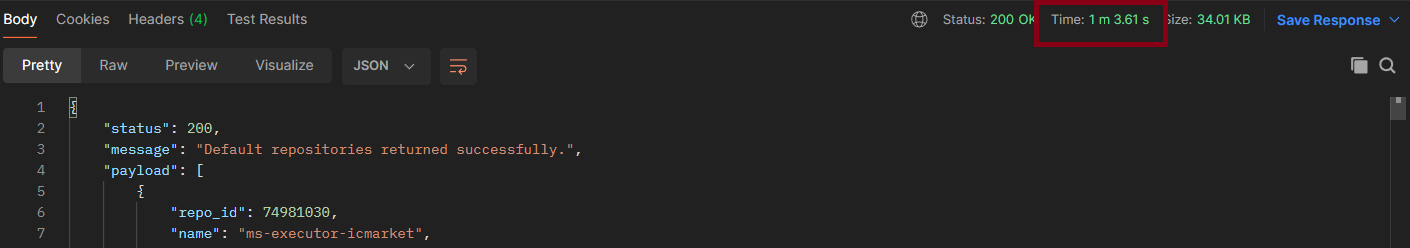
\includegraphics[width=0.8\textwidth]{images/slow.png}
    \caption{Before: Sequential API Calls Causing 30+ Second Load Times}
    \label{fig:gitlab_before}
\end{figure}

\textbf{Solution: Asynchronous Processing and Intelligent Caching}

The solution involved two complementary strategies: implementing asynchronous parallel execution and deploying a multi-layer caching architecture.

\textbf{Part 1: Async/Await for Parallel Execution}

Instead of waiting for each API call to complete before starting the next one, the backend was refactored to use Python's async/await patterns. This enabled parallel execution where all repository data could be fetched simultaneously rather than sequentially. FastAPI's native async support made this implementation straightforward.

The key architectural change transformed the request pattern from:
\begin{itemize}
    \item \textbf{Sequential}: Repo1 → wait → Repo2 → wait → Repo3 → wait (total: sum of all wait times)
    \item \textbf{Parallel}: Repo1, Repo2, Repo3 all fetch simultaneously → wait only once (total: longest single wait time)
\end{itemize}

\textbf{Part 2: Multi-Layer Caching Strategy}

To eliminate redundant API calls and reduce load on GitLab's servers, a sophisticated caching system was implemented:

\begin{itemize}
    \item \textbf{Background Refresh Task}: A background process fetches all repository data every 10 seconds, keeping the cache fresh without waiting for user requests
    \item \textbf{In-Memory Data Structure}: Repository information is stored in fast-access dictionaries, enabling instant O(1) lookup operations
    \item \textbf{Pre-loaded Nested Data}: Each repository object contains pre-loaded pipeline, merge request, and branch data, eliminating the need for additional API calls during user requests
\end{itemize}

This architecture pattern separated data fetching from data serving. The background task handles all external API communication asynchronously, while user-facing API endpoints simply return pre-loaded cached data instantly.

\begin{figure}[H]*
    \centering
    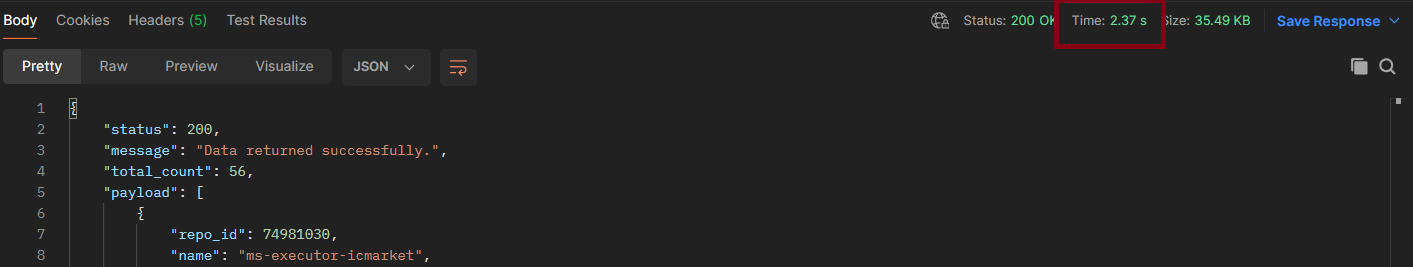
\includegraphics[width=0.8\textwidth]{images/fast.png}
    \caption{After: Async + Caching Resulting in Sub-50ms Response Times}
    \label{fig:gitlab_after}
\end{figure}

\textbf{Performance Results:}

The combined async and caching solution delivered dramatic performance improvements across all measured metrics:

\begin{table}[H]
\centering
\caption{Performance Improvement Results}
\begin{tabular}{|l|l|l|l|}
\hline
\textbf{Metric} & \textbf{Before (Sequential)} & \textbf{After (Async + Cache)} & \textbf{Improvement} \\ \hline
Initial load & 30-80 seconds & 3-5 seconds & 94\% faster \\ \hline
API response & 2-5 seconds & <50ms & 99\% faster \\ \hline
API calls/min & 400+ & 40 (background only) & 90\% reduction \\ \hline
User experience & Frozen UI & Instant updates & \checkmark\ Excellent \\ \hline
Rate limit risk & High & None & \checkmark\ Eliminated \\ \hline
Server load & Heavy & Light & \checkmark\ Optimized \\ \hline
\end{tabular}
\end{table}

\textbf{Key Lessons Learned:}

This challenge highlighted several important principles for building performant web applications:

\begin{itemize}
    \item \textbf{Async is Essential for I/O-Bound Operations}: Network requests should never be executed sequentially when they can be parallelized. Async/await patterns are critical for maintaining responsiveness
    \item \textbf{Cache Intelligently}: Background refresh strategies keep data fresh while eliminating request-time latency. In-memory caching provides instant access without sacrificing data currency
    \item \textbf{Measure, Optimize, Repeat}: Identifying the bottleneck (sequential API calls), implementing a solution (async parallelization), and adding optimization (caching) resulted in near-total performance transformation
\end{itemize}

The solution transformed the Control Panel from a slow, frustrating interface into a responsive, production-ready feature that became the most valued component of the Infrastructure Command Center. The 99\% response time improvement validated the architectural approach and demonstrated the critical importance of performance optimization in user-facing applications.

\section{Conclusion}

This chapter documented the practical implementation of the Infrastructure Command Center, from development environment setup through feature delivery and technical problem-solving. The work environment provided the necessary tools and infrastructure for efficient development, enabling consistent progress across nine two-week sprints.

The solution presentation demonstrated how the three core features Dynamic Visual Workflows, Control Panel, and ML Metrics Monitoring successfully addressed the requirements defined in Chapter 3. Each feature delivered tangible value: the Visual Workflows provided intuitive infrastructure understanding, the Control Panel streamlined repository management and deployment operations, and the ML Metrics Monitoring enabled proactive model performance tracking.

The challenges section highlighted both the learning curve inherent in junior-level development and the technical obstacles that required systematic problem-solving. The React Flow visualization solution and the async/caching performance optimization exemplified how careful technology selection and architectural design directly impact project success. These challenges reinforced the importance of measuring performance, evaluating alternatives objectively, and iterating toward optimal solutions.

The Infrastructure Command Center successfully transformed from architectural designs into a production-deployed platform that centralized FinGenesis's infrastructure management operations, delivering measurable improvements in operational efficiency and user experience.